% =====================================================================
%  U-GNN architecture — orthogonal staircase-U  (reference: oarfish-9)
%  ---------------------------------------------------------------------
%  Builds on the two templates (block_diagram layout + code_A sampling
%  blocks / D_b / bands), with paper-canonical notation (III.3/III.4) and
%  a conditioning bus.  All arrows are horizontal/vertical (90-deg turns);
%  small \sx keeps a tight staircase that reads closer to a U than a V.
%
%  Port convention (no signal/conditioning collisions):
%    encoder block : signal IN west, OUT south ; skip OUT east ; cond IN north
%    decoder block : signal IN south, OUT east ; skip IN west  ; cond IN north
%
%  Notation:
%    encoder   Z_b   = Phi^E_b ( C_b Z_{b-1}, S, D_b ; Theta^E_b, k, Ubar )
%    decoder   Y_{b-1} = Phi^D_b ( [C_b^T Y_b ; Z_b], S, D_{b-1} ; Theta^D_b, k, Ubar )
%    bottleneck Y_B  = Phi^M  ( Z_B, S, D_B ; Theta^M, k, Ubar )
%
%  Compile: pdflatex ugnn_staircase_architecture.tex
% =====================================================================
\documentclass[tikz,border=10pt]{standalone}
\usepackage{amsmath}
\usetikzlibrary{arrows.meta, positioning, calc, backgrounds, fit}

% ===== math macros (edit to match your own preamble) =================
\newcommand{\bbS}{\mathbf{S}}
\newcommand{\bbC}{\mathbf{C}}
\newcommand{\bbD}{\mathbf{D}}
\newcommand{\bbZ}{\mathbf{Z}}
\newcommand{\bbY}{\mathbf{Y}}
\newcommand{\bbU}{\mathbf{U}}
\newcommand{\bbx}{\mathbf{x}}
\newcommand{\Ubar}{\overline{\mathbf{U}}}
\newcommand{\bbeps}{\boldsymbol{\epsilon}_{\boldsymbol{\theta}}}
\newcommand{\rmE}{\mathrm{E}}
\newcommand{\rmD}{\mathrm{D}}
\newcommand{\rmM}{\mathrm{M}}
\newcommand{\PhiE}{\boldsymbol{\Phi}^{\rmE}}
\newcommand{\PhiD}{\boldsymbol{\Phi}^{\rmD}}
\newcommand{\PhiM}{\boldsymbol{\Phi}^{\rmM}}
\newcommand{\Phicond}{\boldsymbol{\Phi}^{\mathrm{cond}}}
\newcommand{\thetaE}{\boldsymbol{\Theta}^{\rmE}}
\newcommand{\thetaD}{\boldsymbol{\Theta}^{\rmD}}
\newcommand{\thetaM}{\boldsymbol{\Theta}^{\rmM}}
\newcommand{\Piin}{\Pi_{\mathrm{in}}}
\newcommand{\Piout}{\Pi_{\mathrm{out}}}

% ---- two-line block display formulas (narrow blocks -> tight staircase) ----
\newcommand{\encform}[1]{$\PhiE_{#1}(\bbC_{#1}\bbZ_{\number\numexpr#1-1\relax},\bbS,\bbD_{#1};$\\$\thetaE_{#1},k,\Ubar)$}
\newcommand{\decform}[1]{$\PhiD_{#1}([\bbC_{#1}^{\top}\bbY_{#1};\bbZ_{#1}],\bbS,\bbD_{\number\numexpr#1-1\relax};$\\$\thetaD_{#1},k,\Ubar)$}
\newcommand{\bottform}{$\PhiM(\bbZ_{\Depth},\bbS,\bbD_{\Depth};$\\$\thetaM,k,\Ubar)$}

% ===== tunable layout parameters =====================================
\def\Depth{3}        % B : number of encoder / decoder levels
\def\sx{2.8}         % horizontal step per depth level (small -> closer to U)
\def\sy{4.0}         % vertical step per depth level (downwards)
\def\Xmax{20.0}      % x-position of the top decoder (right tip of the U)
\def\botdrop{3.5}    % bottleneck drop below the deepest level
\def\railY{5.2}      % height of the conditioning bus rail
\pgfmathsetmacro{\Xc}{\Xmax/2}                       % centre x (bottleneck)
\pgfmathsetmacro{\boty}{2-(\Depth-1)*\sy-\botdrop}   % bottleneck y

\begin{document}
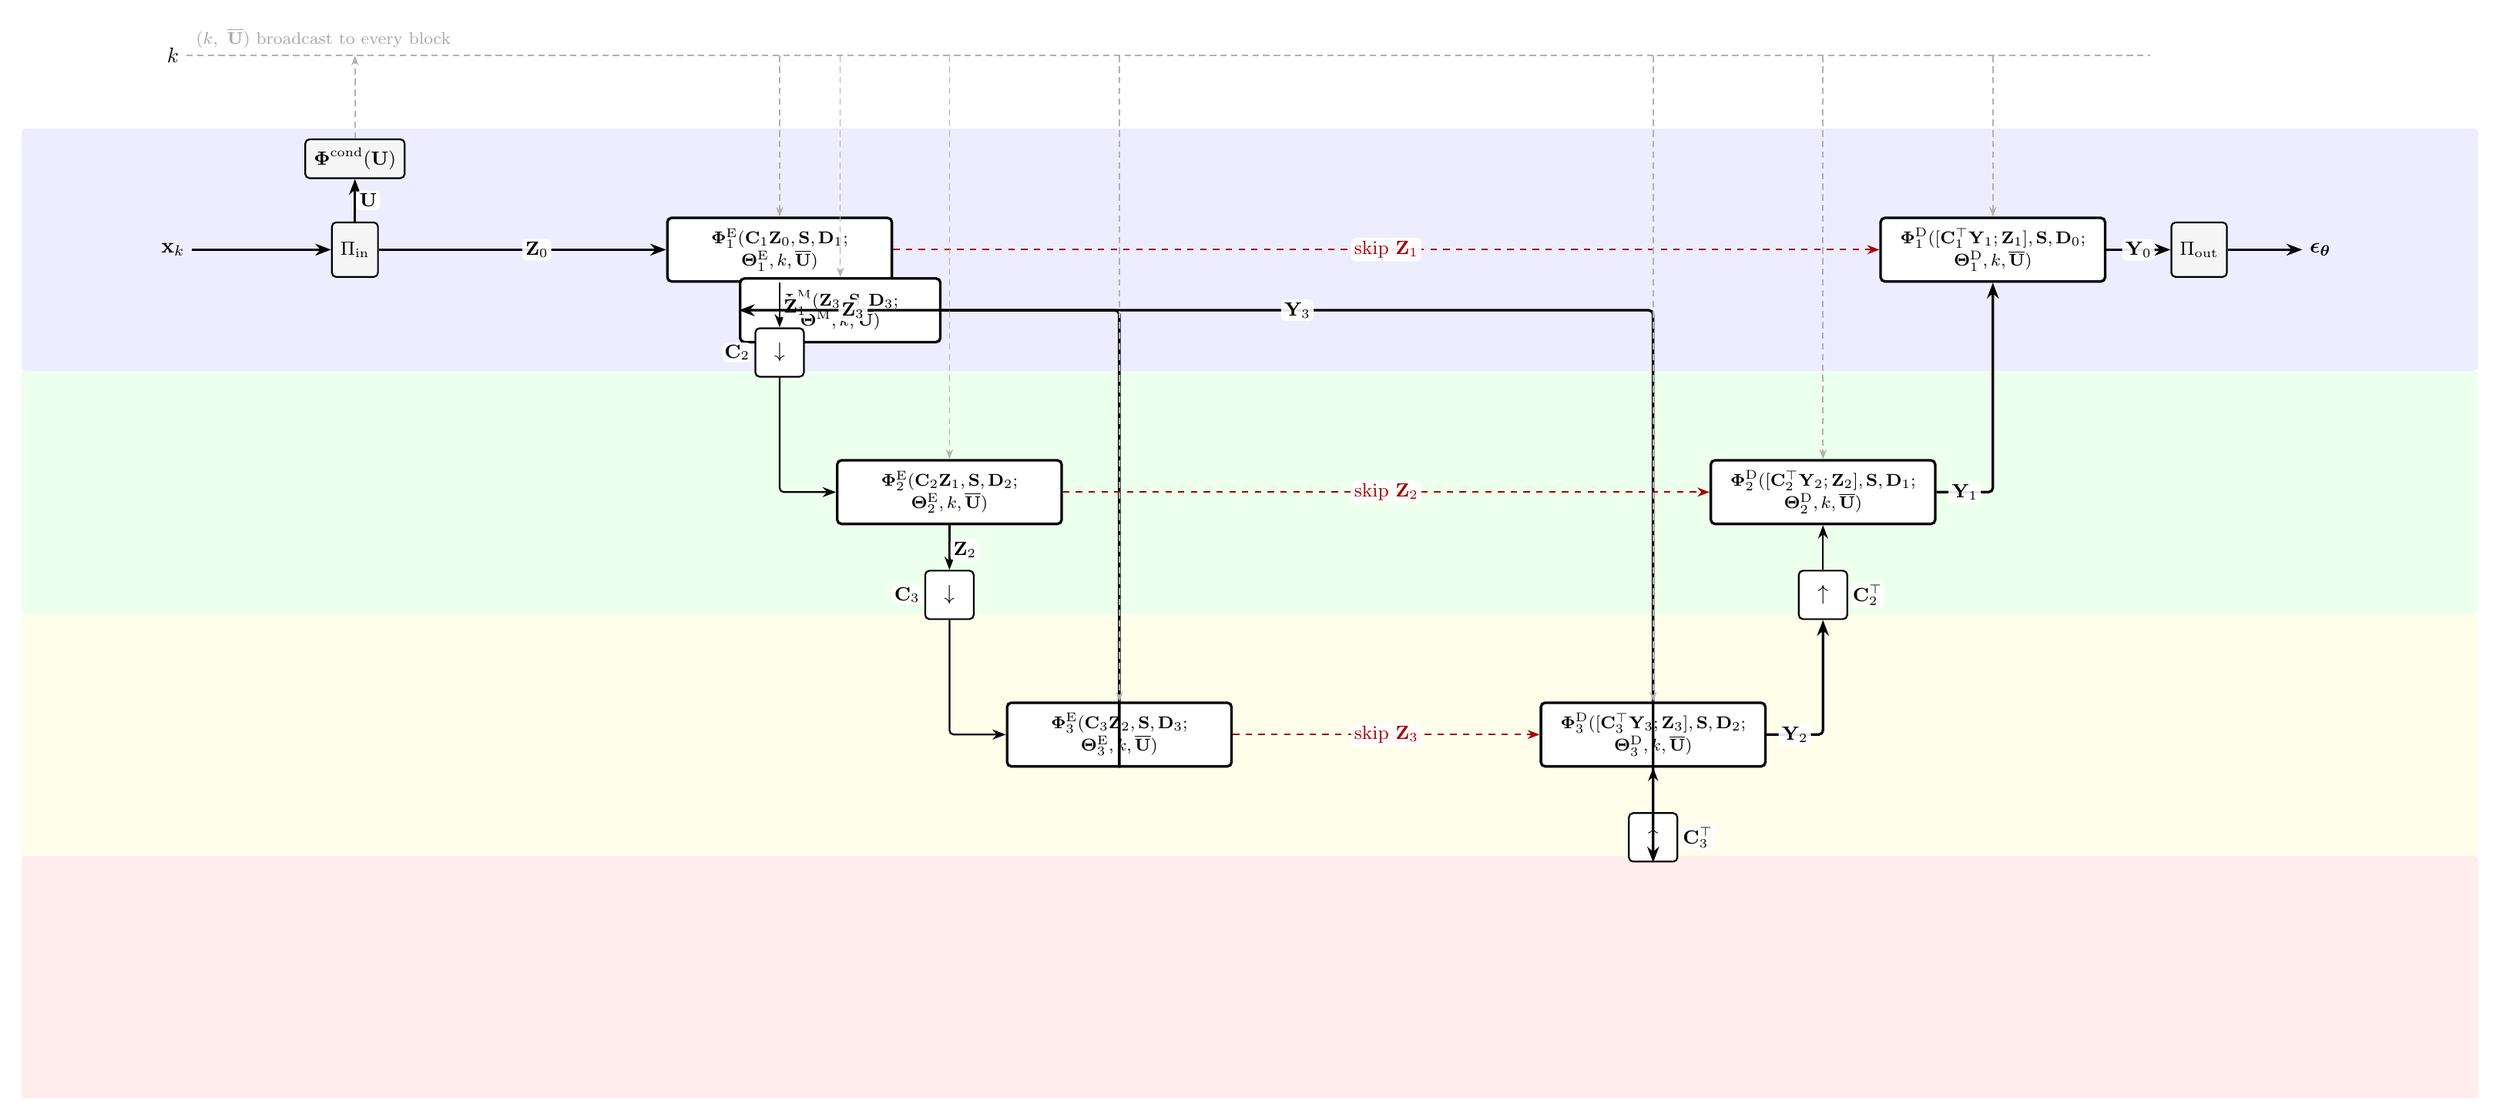
\begin{tikzpicture}[
  >={Stealth[length=2.6mm]},
  rounded corners=2pt,
  block/.style   = {draw, very thick, rounded corners=2pt, align=center,
                    minimum width=3.7cm, minimum height=1.05cm, inner sep=3pt,
                    font=\footnotesize, fill=white},
  bott/.style    = {draw, very thick, rounded corners=2pt, align=center,
                    minimum width=3.3cm, minimum height=1.05cm, inner sep=3pt,
                    font=\footnotesize, fill=white},
  io/.style      = {draw, thick, rounded corners=2pt, align=center,
                    minimum height=0.9cm, inner sep=4pt, font=\small, fill=black!4},
  samp/.style    = {draw, thick, minimum size=0.8cm, inner sep=1pt,
                    font=\normalsize, fill=white},
  cond/.style    = {draw, thick, rounded corners=2pt, align=center,
                    inner sep=4pt, font=\small, fill=black!4},
  sig/.style     = {-{Stealth[length=2.6mm]}, very thick},
  samparr/.style = {-{Stealth[length=2.2mm]}, thick},
  skip/.style    = {-{Stealth[length=2.0mm]}, thick, dashed, red!65!black},
  busln/.style   = {thick, densely dashed, gray!60},
  bustap/.style  = {-{Stealth[length=1.6mm]}, semithick, densely dashed, gray!60},
  elbl/.style    = {font=\small, inner sep=1.5pt, fill=white,
                    fill opacity=0.9, text opacity=1},
  clbl/.style    = {font=\small, inner sep=1pt, fill=white,
                    fill opacity=0.9, text opacity=1},
]

% ---------- encoder & decoder block staircase ----------
\foreach \b in {1,...,\Depth}{
  \pgfmathsetmacro{\ex}{(\b-1)*\sx}
  \pgfmathsetmacro{\ey}{2-(\b-1)*\sy}
  \pgfmathsetmacro{\dx}{\Xmax-(\b-1)*\sx}
  \node[block] (enc-\b) at (\ex,\ey) {\encform{\b}};
  \node[block] (dec-\b) at (\dx,\ey) {\decform{\b}};
}
\node[bott] (bn) at (\Xc,\boty) {\bottform};

% ---------- read-in / read-out / conditioning sources ----------
\node[io]   (pin)  at (-7.0, 2)        {$\Piin$};
\node       (xk)   at (-10.0, 2)       {$\bbx_k$};
\node[cond] (cond) at (-7.0, 3.5)      {$\Phicond(\bbU)$};
\node       (kk)   at (-10.0, \railY)  {$k$};
\node[io]   (pout) at (\Xmax+3.4, 2)   {$\Piout$};
\node       (eps)  at (\Xmax+5.4, 2)   {$\bbeps$};

% ---------- read-in main path ----------
\draw[sig] (xk.east)  -- (pin.west);
\draw[sig] (pin.east) -- (enc-1.west) node[elbl,pos=0.55]{$\bbZ_0$};
\draw[sig] (pin.north) -- (cond.south) node[elbl,pos=0.5,right]{$\bbU$};

% ---------- encoder forward + down-sampling blocks ----------
\foreach \b in {2,...,\Depth}{
  \pgfmathtruncatemacro{\prev}{\b-1}
  \node[samp] (down-\b) at ($(enc-\prev.south)+(0,-1.15)$) {$\downarrow$};
  \node[clbl, left=1pt of down-\b]{$\bbC_{\b}$};
  \draw[samparr] (enc-\prev.south) -- (down-\b.north) node[elbl,pos=0.55,right]{$\bbZ_{\prev}$};
  \draw[samparr] (down-\b.south) |- (enc-\b.west);
}
\draw[sig] (enc-\Depth.south) |- (bn.west) node[elbl,pos=0.85]{$\bbZ_{\Depth}$};

% ---------- decoder forward + up-sampling blocks ----------
% bottleneck -> deepest decoder
\node[samp] (up-\Depth) at ($(dec-\Depth.south)+(0,-1.15)$) {$\uparrow$};
\node[clbl, right=1pt of up-\Depth]{$\bbC_{\Depth}^{\top}$};
\draw[sig]     (bn.east) -| (up-\Depth.south) node[elbl,pos=0.25]{$\bbY_{\Depth}$};
\draw[samparr] (up-\Depth.north) -- (dec-\Depth.south);
% remaining decoder levels
\foreach \b in {\Depth,...,2}{
  \pgfmathtruncatemacro{\prev}{\b-1}
  \ifnum\prev>1
    \node[samp] (up-\prev) at ($(dec-\prev.south)+(0,-1.15)$) {$\uparrow$};
    \node[clbl, right=1pt of up-\prev]{$\bbC_{\prev}^{\top}$};
    \draw[sig]     (dec-\b.east) -| (up-\prev.south) node[elbl,pos=0.25]{$\bbY_{\prev}$};
    \draw[samparr] (up-\prev.north) -- (dec-\prev.south);
  \else
    \draw[sig] (dec-\b.east) -| (dec-\prev.south) node[elbl,pos=0.25]{$\bbY_{\prev}$};
  \fi
}
\draw[sig] (dec-1.east) -- (pout.west) node[elbl,pos=0.5]{$\bbY_0$};
\draw[sig] (pout.east)  -- (eps.west);

% ---------- skip connections  enc_b -> dec_b ----------
\foreach \b in {1,...,\Depth}{
  \draw[skip] (enc-\b.east) -- (dec-\b.west) node[elbl,pos=0.5]{skip $\bbZ_{\b}$};
}

% ---------- conditioning bus (k, Ubar) -> every block ----------
\draw[busln]  (kk.east) -- (\Xmax+2.6,\railY);
\draw[bustap] (cond.north) -- (cond.north|-{(\Xmax,\railY)});
\node[font=\footnotesize, gray!70, above right=0pt and 1pt] at (kk.east)
     {$(k,\ \Ubar)$ broadcast to every block};
\foreach \n in {enc-1,enc-2,enc-3,bn,dec-3,dec-2,dec-1}{
  \draw[bustap] (\n.north |- {(0,\railY)}) -- (\n.north);
}

% ---------- background depth bands ----------
\begin{scope}[on background layer]
  \pgfmathsetmacro{\bandL}{-12.5}
  \pgfmathsetmacro{\bandR}{\Xmax+8.0}
  \foreach \i/\col in {0/blue!7, 1/green!7, 2/yellow!8, 3/red!7}{
    \pgfmathsetmacro{\yt}{2+0.5*\sy-\i*\sy}
    \pgfmathsetmacro{\yb}{\yt-\sy}
    \fill[\col] (\bandL,\yb) rectangle (\bandR,\yt);
  }
\end{scope}

\end{tikzpicture}
\end{document}
